\chapter{Analysis of Improvement Techniques}
\label{cap:analysisOfImprovements}

\noindent This chapter documents the implementation of the following techniques used to improve the chess engine:

\begin{itemize}
    \item Transposition tables with zobrist hashing.
    \item Move generator with magic bitboards and PEXT instructions.
    \item Evaluation with king safety and piece mobility parameters.
    \item Multithread search.
    \item Search with Late move Reductions.
\end{itemize}

\vspace{2em}

\noindent At the end of each section, we provide the results of a 100-game match between the improved engine and a baseline version. The baseline includes only the core techniques discussed in the previous chapter on engine development. The purpose of these matches is to measure the improvement in playing strength introduced by each new implementation.

\vspace{1em}

\noindent All matches are conducted using the tournament manager \textit{CuteChess}~\cite{CuteChess}, with the following configuration:

\begin{itemize}
\item 100 games per match.
\item 50 unique random starting positions, each played twice with alternating colors.
\item 4 seconds of thinking time per move.
\item A 150-move limit per game, after which the game is declared a draw.
\end{itemize}

\newpage

\section{Transposition Table}
\label{sec:tt}

\noindent As discused in the previous chapter (see Section~\ref{chap:iterativeDeepening}), the basic implementation of the chess engine generates a large amount of redundant calculations due to the iterative deepening approach and also the concept of transpositions: situations in which the same board position is reached through different sequences of moves in the game tree.
\noindent Figure~\ref{fig:transposition_example} illustrates a position that can arise through multiple move orders. Where the white king could go to the g3 square from multiple paths.

\begin{figure}[H]
    \centering
    \begin{minipage}{0.6\textwidth}
        \centering
        \newchessgame
        \chessboard[
            showmover=false,
            setfen=8/2k5/3p4/p2P1p2/P2P1P2/8/8/2K5 w - - 0 1,
            pgfstyle=straightmove, color=blue,
            markmoves={c1-e3,e3-g3,c1-g1,g1-g3},
            arrow=to
        ]
    \end{minipage}
    \caption{Lasker-Reichhelm Position, transposition example}
    \label{fig:transposition_example}
\end{figure}

\vspace{1em}

\noindent Taking advantage of the concept of dynamic programming, we create a look-up table of chess positions and its evaluation. So if we encounter the same position again, the evaluation is already precalculated. However, we ask ourselves the following question: how much space does the look-up table take up if there are an astronomical amount of chess positions? What we can do is assign a hash to each position and make the table index the last bits of the hash. The larger the table, the less likely access collisions will be. We also want a hash that is fast to calculate and has collision-reducing properties.
~\cite{TranspositionTable}

\vspace{1em}

\noindent The complete implementation can be found in the following file:\\
\scriptsize\url{https://github.com/LauraWangQiu/AlphaDeepChess/blob/main/include/utilities/transposition_table.hpp}\normalsize.

\vspace{2em}

\subsection*{Zobrist Hashing}

Zobrist Hashing is a technique to transform a board position of arbitrary size into a number of a set length, with an equal distribution over all possible numbers invented by Albert Zobrist. (\cite{ZobristHashing})

\vspace{1em}

To generate a 64-bit hash for a position, the following steps are followed:

\begin{enumerate}
  \item Pseudorandom 64-bit numbers are generated for each possible feature of a position:
  \begin{enumerate}
    \item One number for each piece type on each square — 12 pieces x 64 squares = 768 numbers.
    \item One number to indicate the side to move is black.
    \item Four numbers to represent castling rights (kingside and queenside for both white and black).
    \item Eight numbers to represent the file of an available en passant square.
  \end{enumerate}
  \item The final hash is computed by XOR-ing together all the random numbers corresponding to the features present in the current position.
\end{enumerate}

\vspace{1em}

\noindent These random values ensure that even slightly different positions produce very different hash values. This greatly reduces the chance of collisions.

\vspace{1em}

\noindent The XOR operation is used not only because it is computationally inexpensive, but also because it is reversible. This means that when a move is made or undone, we can update the hash incrementally by applying XOR only to the affected squares, without needing to recompute the entire hash.

\vspace{1em}

The position shown in Figure~\ref{fig:zobristExamplePosition} illustrates an example of how the Zobrist hash is computed.  
The hash value is calculated by XORing the random values associated with each element of the position.  
Since the side to move is White, we do not XOR the value associated with Black to move.  
The resulting hash is computed as follows:

\[
111 \oplus 69 \oplus 909 \oplus 10 \oplus 67 \oplus 12 \oplus 555 \oplus 3 = 458
\]

\begin{figure}[H]
    \begin{minipage}{0.4\textwidth}
        \centering
        \newchessgame
        \chessboard[
            showmover=true,
            setfen=7r/8/k7/1pP5/8/4Q3/1P6/1K6 w - b6 0 1,
            markstyle=circle,
            color=blue, markfields={b6},
            pgfstyle=straightmove, color=red,
            markmoves={b7-b5},
            arrow=to
        ]
        \caption*{Side to move is white. The last move was a pawn advancing from b7 to b5, making en passant available on the b6 square.}
    \end{minipage}
    \hfill
    \begin{minipage}{0.4\textwidth}
        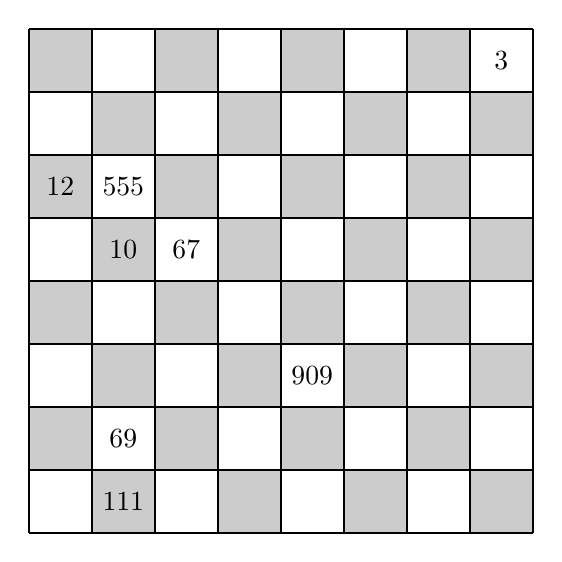
\begin{tikzpicture}[scale=0.8]

            \foreach \x in {0,1,...,7} {
                \foreach \y in {0,1,...,7} {
                    \pgfmathparse{mod(\x+\y,2) ? "black!20" : "white"}
                    \edef\col{\pgfmathresult}
                    \fill[\col] (\x,\y) rectangle (\x+1,\y+1);
                }
            }

            \node at (1.5,0.5) {111}; \node at (1.5,1.5) {69}; \node at (4.5,2.5) {909}; \node at (1.5,4.5) {10};
            \node at (2.5,4.5) {67}; \node at (0.5,5.5) {12}; \node at (1.5,5.5) {555}; \node at (7.5,7.5) {3};

            \draw[thick] (0,0) grid (8,8);
        \end{tikzpicture}
        \caption*{Random values corresponding to each piece and the en passant square. The value for Black to move is 62319.}    \end{minipage}
    \caption{Zobrist hash calculation example}
    \label{fig:zobristExamplePosition}
\end{figure}

\subsection*{Table Entry}

Each entry in the transposition table stores the following information:

\begin{enumerate}
  \item Zobrist Hash: The full 64-bit hash of the position. This is used to verify that the entry corresponds to the current position and to detect possible index collisions in the table.
  \item Evaluation: The numerical evaluation of the position, as computed by the evaluation function.
  \item Depth: The depth at which the evaluation was calculated. A deeper search could potentially yield a more accurate evaluation, so this value helps determine whether a new evaluation should overwrite the existing one.
  \item Node Type: Indicates the type of node stored:
  \begin{enumerate}
    \item \textit{EXACT} the evaluation is precise for this position.
    \item \textit{UPPERBOUND} the evaluation is an upper bound, typically resulting from an alpha cutoff.
    \item \textit{LOWERBOUND} the evaluation is a lower bound, typically resulting from a beta cutoff.
    \item \textit{FAILED} entry is empty or with invalid information.
  \end{enumerate}
\end{enumerate}

\subsection*{Collisions}

As discussed earlier, index collisions in the transposition table are handled by verifying the full Zobrist hash stored in the entry. However, it is still theoretically possible for a full hash collision to occur, that is two different positions producing the same hash.

\vspace{1em}

\noindent This scenario is extremely rare. With 64-bit hashes, there are $2^{64}$ possible unique values, which is more than sufficient for practical purposes. In the unlikely event of a true hash collision, it could result in an incorrect evaluation being reused for a different position.

\subsection*{Analysis}

\noindent To evaluate the impact of introducing the transposition table, we conducted the 100-game tournament against the baseline version of the engine. The Table ~\ref{tab:tt_vs_basic} details the implementation used for each bot.

\begin{table}[H]
    \centering
    \caption{Match configuration: Transposition Table Bot vs Basic Bot}
    \label{tab:tt_vs_basic}
    \begin{tabular}{|l|c|c|}
    \hline
    \textbf{Component}         & \textbf{Transposition Table Bot}  & \textbf{Basic Bot}     \\ \hline
    Search                     & Alpha-beta With Transposition Table          & Basic Alpha-beta           \\ \hline
    Evaluation Function        & Materialistic                      & Materialistic       \\ \hline
    Move Generator             & Basic implementation              & Basic implementation   \\ \hline
    Move Ordering              & MVV-LVA                           & MVV-LVA                \\ \hline
    \end{tabular}
\end{table}

\noindent As illustrated in Figure~\ref{fig:results_transposition_table_bot}, We see a substantial improvement by adding the transposition table with 46 wins versus 32 losses. The remaining 22 games ended in a draw.

\begin{center}
\begin{figure}[H]
    \centering
    \ResultBar{15cm}{0.5cm}{46}{22}{32}
    \caption{64MB Transposition Table bot vs basic bot}
    \label{fig:results_transposition_table_bot}
\end{figure}
\medskip
\end{center}

\section{Move generator with Magic Bitboards and PEXT instructions}

To identify potential performance bottlenecks, we performed profiling on the engine, as shown in Figure~\ref{fig:profiling}.

\begin{center}
    \begin{figure}[H]
    \centering
        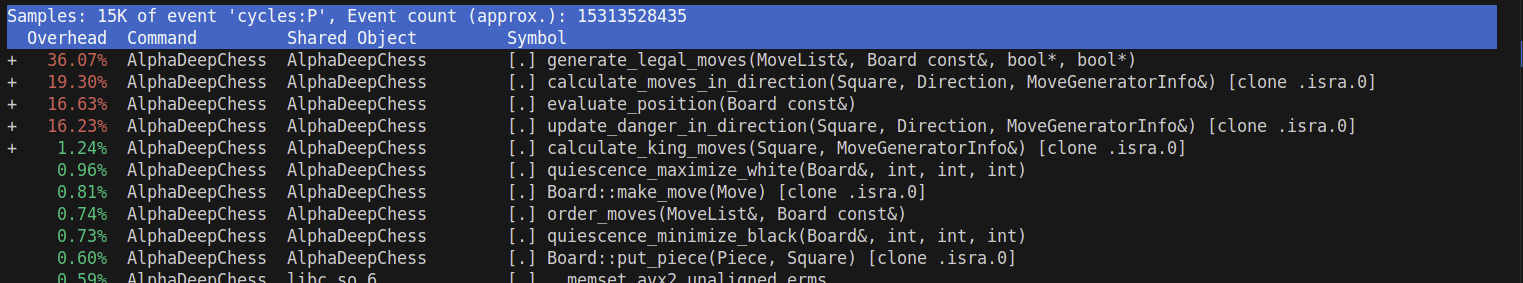
\includegraphics[width=1.0\textwidth]{Imagenes/basic_move_generator_profiling.png}
        \caption{Profiling results}
        \label{fig:profiling}
    \end{figure}
    \medskip
\end{center}

\noindent The profiling results indicate that the majority of the total execution time is spent in the legal move generation function. Therefore, optimizing this component is expected to yield significant performance improvements.

\subsection*{Magic bitboards}

We can create a look up table of all the rook and bishop moves for each square on the board and for each combination of pieces that blocks the path of the slider piece (blockers  bitboard). Basically we need a hash table to store rook and bishop moves indexed by square and bitboard of blockers. The problem is that this table could be very big.~\cite{MagicBitboards}

\vspace{1em}

\noindent Magic bitboards technique used to reduce the size of the look up table. We cut off unnecesary information in the blockers bitboard, excluding the board borders and the squares outside its attack pattern.

\vspace{1em}

A \textbf{magic number} is a multiplier to the bitboard of blockers with the following properties:

\begin{itemize}
  \item Preserves relevant blocker information: 
  The nearest blockers along a piece's movement direction are preserved. 
  \textit{Example:} Consider a rook with two pawns in its path:
  \begin{lstlisting}[breaklines=true]
    Rook -> -> -> [Pawn1][Pawn2]
  \end{lstlisting}
  In this case, only `Pawn1` blocks the rook's movement, while `Pawn2` is irrelevant.
  \item Compresses the blocker bitboard, pushing the important bits near the most significant bit.
  \item The final multiplication must produce a unique index for each possible blocker configuration. The way to ensure the uniqueness is by brute force testing.
\end{itemize}

\noindent As illustrated in Figure~\ref{fig:magics_position}, we aim to compute the legal moves of the white rook in the given position. In practice, the only pieces that truly block the rook's path are those marked with a red circle.

\begin{figure}[H]
    \centering
    \begin{minipage}{0.6\textwidth}
        \centering
        \newchessgame
        \chessboard[
            showmover=false,
            setfen=n1bk3r/3p4/1p1p2p1/8/3R1p2/8/3p4/7n w - - 0 1,
            markstyle=circle,
            color=red, markfields={d6,f4,d2},
            color=green, markfields={c4,b4,a4,e4,d5,d3}
        ]
    \end{minipage}
    \caption{Initial chess position with white rook and blockers}
    \label{fig:magics_position}
\end{figure}

\noindent First, we mask out all pieces outside the rook's attack pattern or on the board borders, as shown in Figure~\ref{fig:magic_preprocessing}.

\begin{figure}[H]
    \centering
    \begin{minipage}[c]{0.4\textwidth}
        \centering
        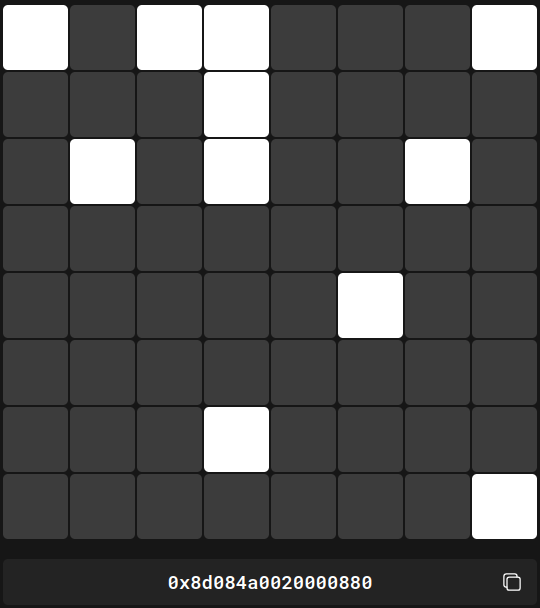
\includegraphics[width=\textwidth]{Imagenes/magics_blockers.png}
        \caption*{Original blockers bitboard}
    \end{minipage}
    \hfill
    \begin{minipage}[c]{0.1\textwidth}
        \centering
        \small$\to$
    \end{minipage}
    \hfill
    \begin{minipage}[c]{0.4\textwidth}
        \centering
        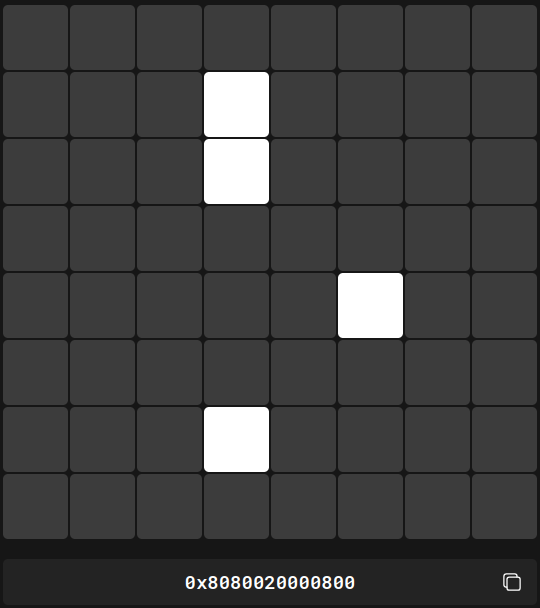
\includegraphics[width=\textwidth]{Imagenes/magics_processed_blockers.png}
        \caption*{Masked blockers bitboard}
    \end{minipage}
    \caption{Pre-processing of the blockers bitboard}
    \label{fig:magic_preprocessing}
\end{figure}

\noindent As illustrated in Figure~\ref{fig:magic_multiplication}, the masked blockers bitboard is then multiplied by the magic number. The result retains only the three relevant pawns that obstruct the rook's movement, pushing them toward the most significant bits.

\begin{figure}[H]
    \centering
    \begin{minipage}[c]{0.4\textwidth}
        \centering
        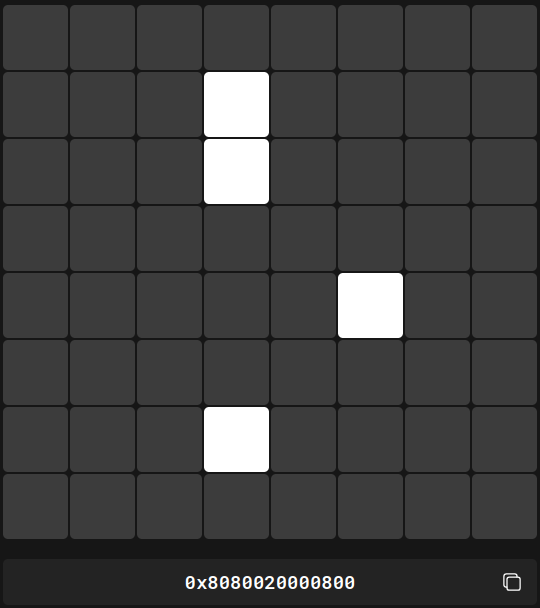
\includegraphics[width=\textwidth]{Imagenes/magics_processed_blockers.png}
        \caption*{Masked blockers bitboard}
    \end{minipage}
    \hfill
    \begin{minipage}[c]{0.1\textwidth}
        \centering
        \Huge$\times$ \\[0.5em]
        \small Magic number \\[0.5em]
        \Huge$=$
    \end{minipage}
    \hfill
    \begin{minipage}[c]{0.4\textwidth}
        \centering
        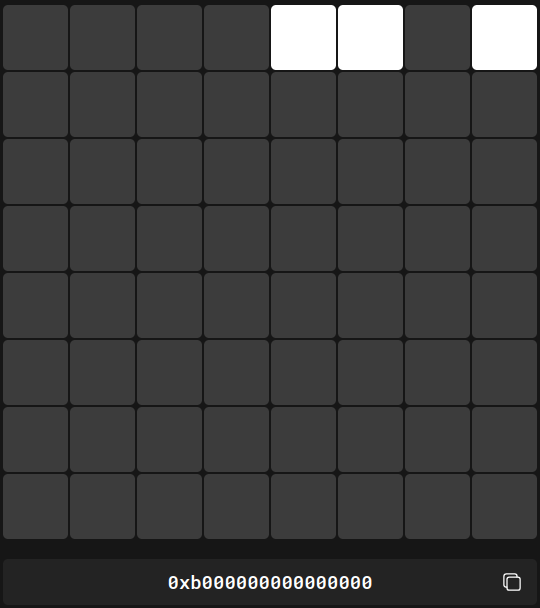
\includegraphics[width=\textwidth]{Imagenes/magics_multiplied_blockers.png}
        \caption*{Multiplied blockers bitboard}
    \end{minipage}
    \caption{Multiplication by magic number to produce an index}
    \label{fig:magic_multiplication}
\end{figure}

\noindent Next, we compress the index toward the least significant bits by shifting right by \(\,64-\)\texttt{relevant\_squares}. The number of relevant squares varies per board square; Listing~\ref{fig:rook_relevant_squares} shows this for the rook:

\begin{figure}[H]
    \centering
    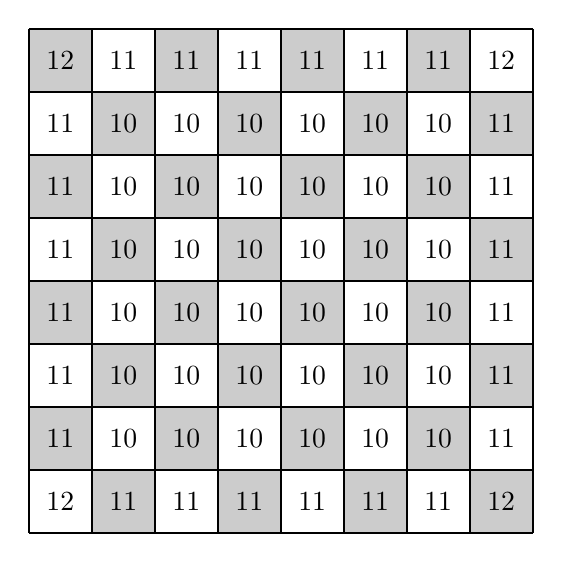
\begin{tikzpicture}[scale=0.8]
        % Draw the chessboard
        \foreach \x in {0,1,...,7} {
            \foreach \y in {0,1,...,7} {
                \pgfmathparse{mod(\x+\y,2) ? "black!20" : "white"}
                \edef\col{\pgfmathresult}
                \fill[\col] (\x,\y) rectangle (\x+1,\y+1);
            }
        }

        % Add the values to the squares
        \node at (0.5,7.5) {12}; \node at (1.5,7.5) {11}; \node at (2.5,7.5) {11}; \node at (3.5,7.5) {11};
        \node at (4.5,7.5) {11}; \node at (5.5,7.5) {11}; \node at (6.5,7.5) {11}; \node at (7.5,7.5) {12};

        \node at (0.5,6.5) {11}; \node at (1.5,6.5) {10}; \node at (2.5,6.5) {10}; \node at (3.5,6.5) {10};
        \node at (4.5,6.5) {10}; \node at (5.5,6.5) {10}; \node at (6.5,6.5) {10}; \node at (7.5,6.5) {11};

        \node at (0.5,5.5) {11}; \node at (1.5,5.5) {10}; \node at (2.5,5.5) {10}; \node at (3.5,5.5) {10};
        \node at (4.5,5.5) {10}; \node at (5.5,5.5) {10}; \node at (6.5,5.5) {10}; \node at (7.5,5.5) {11};

        \node at (0.5,4.5) {11}; \node at (1.5,4.5) {10}; \node at (2.5,4.5) {10}; \node at (3.5,4.5) {10};
        \node at (4.5,4.5) {10}; \node at (5.5,4.5) {10}; \node at (6.5,4.5) {10}; \node at (7.5,4.5) {11};

        \node at (0.5,3.5) {11}; \node at (1.5,3.5) {10}; \node at (2.5,3.5) {10}; \node at (3.5,3.5) {10};
        \node at (4.5,3.5) {10}; \node at (5.5,3.5) {10}; \node at (6.5,3.5) {10}; \node at (7.5,3.5) {11};

        \node at (0.5,2.5) {11}; \node at (1.5,2.5) {10}; \node at (2.5,2.5) {10}; \node at (3.5,2.5) {10};
        \node at (4.5,2.5) {10}; \node at (5.5,2.5) {10}; \node at (6.5,2.5) {10}; \node at (7.5,2.5) {11};

        \node at (0.5,1.5) {11}; \node at (1.5,1.5) {10}; \node at (2.5,1.5) {10}; \node at (3.5,1.5) {10};
        \node at (4.5,1.5) {10}; \node at (5.5,1.5) {10}; \node at (6.5,1.5) {10}; \node at (7.5,1.5) {11};

        \node at (0.5,0.5) {12}; \node at (1.5,0.5) {11}; \node at (2.5,0.5) {11}; \node at (3.5,0.5) {11};
        \node at (4.5,0.5) {11}; \node at (5.5,0.5) {11}; \node at (6.5,0.5) {11}; \node at (7.5,0.5) {12};

        % Draw the grid
        \draw[thick] (0,0) grid (8,8);
    \end{tikzpicture}
    \caption{Relevant squares for rook piece.}
    \label{fig:rook_relevant_squares}
\end{figure}

\vspace{1em}

\noindent The final index is thus computed as:

\begin{align*}
    \text{index}
    &= (\texttt{bitboard\_of\_blockers} \times \texttt{magic\_number})
       \;\gg\;(64 - \texttt{relevant\_squares})\,.
\end{align*}

\subsection*{PEXT instruction}

\noindent The \texttt{PEXT} (Parallel Bits Extract) instruction—available on modern x86\_64 CPUs—extracts bits from a source operand according to a mask and packs them into the lower bits of the destination operand.~\cite{PextInstruction} It is ideally suited for computing our table index.

Figure~\ref{fig:pext_instruction_example} illustrates how \texttt{PEXT} works: it selects specific bits from register \texttt{r2}, as specified by the mask in \texttt{r3}, and packs the result into the lower bits of the destination register \texttt{r1}.

\begin{figure}[H]
    \centering
    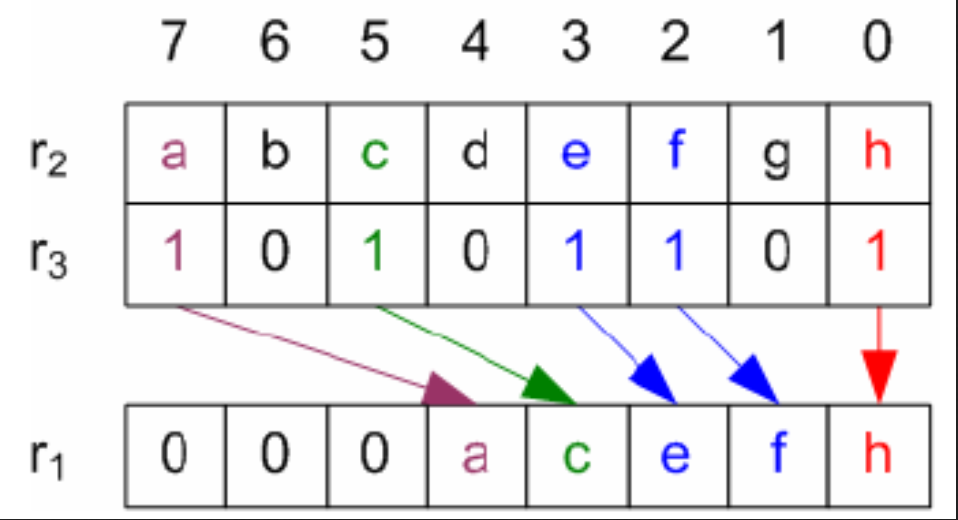
\includegraphics[width=0.5\textwidth]{Imagenes/pext.png}
    \caption{Example of the \texttt{PEXT} instruction: extracting bits from \texttt{r2} using \texttt{r3} as a mask, and storing the result in \texttt{r1}. ~\cite{PextInstruction}}
    \label{fig:pext_instruction_example}
\end{figure}

\noindent For our previous example (see Figure~\ref{fig:magics_position}), we only need the full bitboard of blockers and the rook’s attack pattern (excluding the borders to reduce space), as illustrated in Figure~\ref{fig:pext_bitboards}.

\begin{figure}[H]
    \centering
    \begin{minipage}[c]{0.3\textwidth}
        \centering
        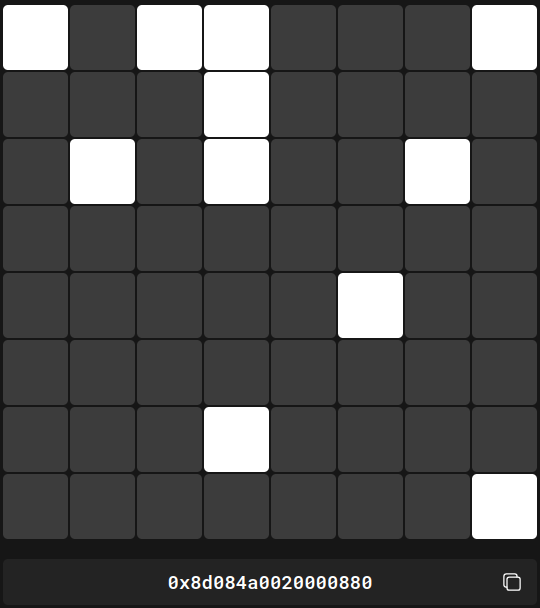
\includegraphics[width=\textwidth]{Imagenes/magics_blockers.png}
        \caption*{Blockers bitboard}
    \end{minipage}
    \hfill
    \begin{minipage}[c]{0.3\textwidth}
        \centering
        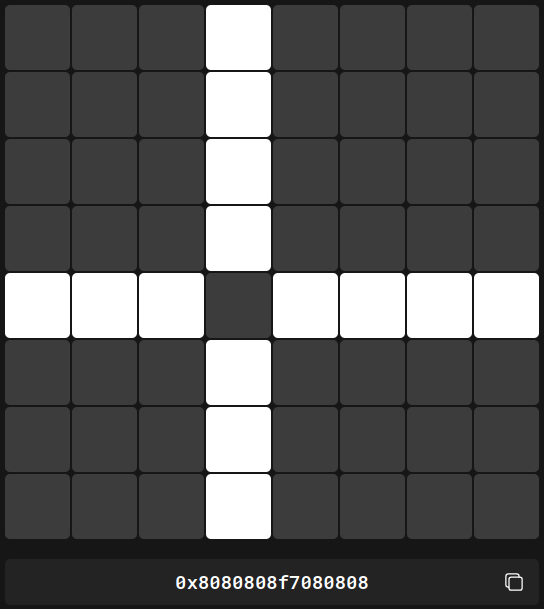
\includegraphics[width=\textwidth]{Imagenes/magics_rook_attacks.png}
        \caption*{Rook attack mask}
    \end{minipage}
    \hfill
    \begin{minipage}[c]{0.05\textwidth}
        \centering
        \Huge\texttt{->}
    \end{minipage}
    \hfill
    \begin{minipage}[c]{0.3\textwidth}
        \centering
        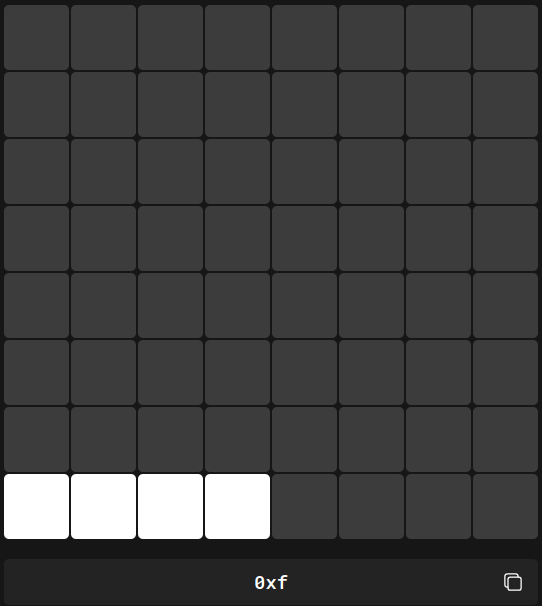
\includegraphics[width=\textwidth]{Imagenes/pext_final_index.png}
        \caption*{Final extracted index}
    \end{minipage}
    \caption{index extraction with Pext example}
    \label{fig:pext_bitboards}
\end{figure}

\noindent The final index used to access the lookup table is calculated using the \texttt{pext} instruction as follows:

\begin{align*}
    \text{index}
    &= \texttt{\_pext\_u64}(\texttt{blockers},\,\texttt{attack\_pattern})\,.
\end{align*}

\noindent To maintain compatibility and performance across different hardware platforms, we provide two implementations:

\begin{itemize}
  \item If \texttt{PEXT} support is detected at compile time, the engine uses it to compute the index directly.
  \item Otherwise, the engine falls back to the Magic Bitboards approach using multiplication and bit shifts.
\end{itemize}

\subsection*{Analysis}

\noindent To evaluate the impact of introducing the move generator accelerated with pext instructions, we conducted the 100-game tournament against the baseline version of the engine. The Table ~\ref{tab:pext_vs_basic} details the implementation used for each bot.

\begin{table}[H]
    \centering
    \caption{Match configuration: PEXT instructions Bot vs Basic Bot}
    \label{tab:pext_vs_basic}
    \begin{tabular}{|l|c|c|}
    \hline
    \textbf{Component}         & \textbf{PEXT instructions Bot}  & \textbf{Basic Bot}     \\ \hline
    Search                     & Alpha-beta With Transposition Table          & Basic Alpha-beta           \\ \hline
    Evaluation Function        & Materialistic                      & Materialistic       \\ \hline
    Move Generator             & PEXT implementation              & Basic implementation   \\ \hline
    Move Ordering              & MVV-LVA                           & MVV-LVA                \\ \hline
    \end{tabular}
\end{table}

\noindent As illustrated in Figure~\ref{fig:results_pext_move_generator_bot}, We achieved a significant performance improvement by adding the PEXT instructions with 46 wins versus 22 losses. The remaining 14 games ended in a draw.

\begin{center}
    \begin{figure}[H]
        \centering
        \ResultBar{15cm}{0.5cm}{64}{14}{22}
        \caption{Move generator with PEXT instructions bot vs basic bot}
        \label{fig:results_pext_move_generator_bot}
    \end{figure}
\medskip
\end{center}

\section{Evaluation with King Safety and piece mobility}

It is often beneficial to evaluate additional aspects of a position beyond simply counting material. We introduce the following positional evaluation parameters:

\begin{enumerate}
    \item King Shield Bonus: The king is typically safer when protected by friendly pawns in front of it. We assign a bonus in the evaluation score for each allied pawn positioned directly in front of the king.

    \item King Safety Penalty: For each square within a $3 \times 3$ area surrounding the king that is attacked by enemy pieces, we apply a penalty to reflect increased vulnerability.

    \item Piece Mobility: Greater piece mobility is generally indicative of a stronger position. Each piece receives a bonus for every available move to a square that is not attacked by enemy pawns.
\end{enumerate}

\subsection*{Analysis}

\noindent To evaluate the impact of introducing the new parameters in the evaluation, we conducted the 100-game tournament against the baseline version of the engine. The Table ~\ref{tab:safety_mobility_vs_basic} details the implementation used for each bot.

\begin{table}[H]
    \centering
    \caption{Match configuration: King Safety and Piece mobility eval Bot vs Basic Bot}
    \label{tab:safety_mobility_vs_basic}
    \begin{tabular}{|l|c|c|}
    \hline
    \textbf{Component}         & \textbf{PEXT instructions Bot}  & \textbf{Basic Bot}     \\ \hline
    Search                     & Alpha-beta With Transposition Table          & Basic Alpha-beta           \\ \hline
    Evaluation Function        & Safety and Mobility                      & Materialistic      \\ \hline
    Move Generator             & PEXT implementation              & Basic implementation   \\ \hline
    Move Ordering              & MVV-LVA                           & MVV-LVA                \\ \hline
    \end{tabular}
\end{table}

\noindent As illustrated in Figure~\ref{fig:results_safety_mobility_bot}, the results are slightly worse compared to the match using the material-only evaluation shown in Figure~\ref{fig:results_pext_move_generator_bot}, with 62 wins and 30 losses. This decline may be attributed to the additional computational overhead introduced by evaluating the new parameters. Moreover, while concepts such as king safety and piece mobility are intuitively valuable to human players, the engine may struggle to consistently associate them with actual positional strength.

\vspace{1em}

\begin{center}
    \begin{figure}[H]
        \centering
        \ResultBar{15cm}{0.5cm}{62}{8}{30}
        \caption{King Safety and Piece mobility evaluation bot vs basic bot}
        \label{fig:results_safety_mobility_bot}
    \end{figure}
\medskip
\end{center}

\section{Search Multithread}
TODO
%
%This version of search follows YBWC mentioned in Section~\ref{sec:alphabetaEnhancements}. It searches the first move sequentially after ordering the moves and launches the remaining moves in parallel using a thread. If it turns out that the first move was the best and pruning was applied, directly return the final node evaluation without the additional thread.
%
%\paragraph{Young Brothers Wait Concept} is a parallel search algorithm designed to optimize the distribution of work among multiple threads. This is particularly effective in alpha-beta pruning, where the search tree is explored selectively. It is divided into two phases: the principal variation move and the wait concept. The principal variation is searched sequentially by the main thread which ensures that the most promising move is evaluated first. Then, once the first move is evaluated, the remaining moves are distributed among multiple threads for parallel evaluation.
%
%\begin{figure}[H]
%    \centering
%    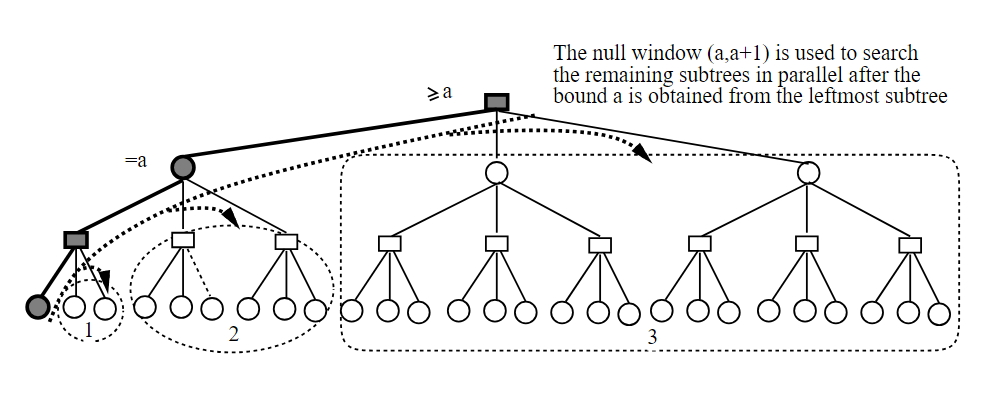
\includegraphics[width=0.8\textwidth]{Imagenes/Bitmap/pvsplitting.png}
%    \caption{Principal variation splitting.~\cite{PVSplitting}}
%    \label{fig:pv-splitting}
%\end{figure}
%
%\subsection*{Analysis}

%To evaluate the improvement in the new evaluation, we conducted the same 100 game match vs the basic bot version. 
%
%\begin{center}
%    \begin{figure}[H]
%        \centering
%        \ResultBar{15cm}{0.5cm}{32}{5}{63}
%        \caption{Multithread Search bot vs basic bot}
%        \label{fig:results_multithread_search_bot}
%    \end{figure}
%\medskip
%\end{center}
%
%\noindent The results are slightly worse compared to the match using the material-only evaluation, with 8 more losses than before. This may be due to the increased computational cost of evaluating these additional parameters. Furthermore, although these are abstract concepts commonly used by humans to assess positions, the engine may struggle to find a clear correlation between them and actual positional strength.
%
\section{Late Move Reductions}
TODO
%We experiment with the use of late move pruning, under the assumption that if our move ordering is good, the best move in the position should be among the first explored moves. We reduce the depth by one unit starting from the tenth movement.
%
%\subsection*{Analysis}
%
%To evaluate the improvement in the new evaluation, we conducted the same 100 game match vs the basic bot version.
%
%\begin{center}
%    \begin{figure}[H]
%        \centering
%        \ResultBar{15cm}{0.5cm}{48}{15}{37}
%        \caption{Reductions Search bot vs basic bot}
%        \label{fig:results_reductions_search_bot}
%    \end{figure}
%\medskip
%\end{center}
%
%\noindent The results are worse, with 15 more losses than the version without this aggresive pruning.~\ref{fig:results_pext_move_generator_bot} This could be because our move ordering is not that strong, and the best move in the position sometimes is in the last positions.